\documentclass{thapathaliece}

% --- FONT CONFIGURATION ---
% Explicitly setting the fonts to match common IOE requirements
\usepackage[T1]{fontenc}
\usepackage{newtxtext,newtxmath} % Standard Times font for engineering

% --- PROJECT DATA ---
\newcommand{\cProjectTitle}{FINE-TUNING OF LLAMA-2 7B FOR PYTHON CODE GENERATION}
\newcommand{\cProjectType}{A Project Proposal}
\newcommand{\cSupervisor}{[Supervisor Name]} 
\newcommand{\cDepartment}{Department of Electronics and Computer Engineering}
\newcommand{\cMonth}{February}
\newcommand{\cYear}{2026}

\renewcommand{\cSubmittedI}{Deep Shrestha}
\renewcommand{\cSubmittedIRoll}{THA079BCT011}
\renewcommand{\cSubmittedII}{Pradip Pokhrel}
\renewcommand{\cSubmittedIIRoll}{THA079BCT027}
\renewcommand{\cSubmittedIII}{Rohan Dhakal}
\renewcommand{\cSubmittedIIIRoll}{THA079BCT033}
\renewcommand{\cSubmittedIV}{Sanjay Shrestha}
\renewcommand{\cSubmittedIVRoll}{THA079BCT039}

\makeglossaries

\begin{document}

% 1. TITLE PAGE (No page number)
\begin{titlepage}
    \thispagestyle{empty}
    \begin{center}
        \includegraphics[width=1.5in]{logo.png}\\[0.4cm]
        {\large \textbf{TRIBHUVAN UNIVERSITY}}\\[0.1cm]
        {\large \textbf{INSTITUTE OF ENGINEERING}}\\[0.1cm]
        {\large \textbf{THAPATHALI CAMPUS}}\\[2cm]
        
        {\large \textbf{\cProjectType}}\\[0.1cm]
        {\large \textbf{ON}}\\[0.1cm]
        {\large \textbf{\cProjectTitle}}\\[2cm]
        
        {\large \textbf{SUBMITTED BY:}}\\[0.4cm]
        \begin{tabular}{ll}
            \cSubmittedI & (\cSubmittedIRoll) \\
            \cSubmittedII & (\cSubmittedIIRoll) \\
            \cSubmittedIII & (\cSubmittedIIIRoll) \\
            \cSubmittedIV & (\cSubmittedIVRoll) \\
        \end{tabular}\\[2cm]
        
        {\large \textbf{SUBMITTED TO:}}\\[0.1cm]
        {\cDepartment}\\[0.1cm]
        {Thapathali Campus, Kathmandu, Nepal}\\[2cm]
        
        {\cMonth, \cYear}
    \end{center}
\end{titlepage}

% 2. FRONT MATTER (Roman numerals start here)
\cleardoublepage
\pagenumbering{roman}
\setcounter{page}{1}

% Use \phantomsection and \addcontentsline to ensure TOC links work with hyperref
\cleardoublepage
\phantomsection
\addcontentsline{toc}{chapter}{ACKNOWLEDGEMENT}
\chapter*{ACKNOWLEDGEMENT}
% No need for \addcontentsline; KOMA-script classes usually handle this 
% or the main.tex handles the TOC entry for the front matter.

\onehalfspacing % Matches the campus 1.5 line spacing requirement

We would like to express our sincere gratitude to the Department of Electronics and Computer Engineering, Thapathali Campus, and Asst. Prof. Suwarna Lingden, for his invaluable guidance, encouragement, and insightful feedback that greatly enhanced the quality of our work. We extend our heartfelt thanks to all those who have supported and guided us throughout the process of preparing this project proposal.

\vspace{1.5cm}

\noindent
\textbf{Submitted By:}\\
\authorTable 
% Using \authorTable ensures the names and roll numbers align perfectly 
% as defined in your .cls file.

\cleardoublepage
\phantomsection
\addcontentsline{toc}{chapter}{ABSTRACT}
\chapter*{ABSTRACT}
\addcontentsline{toc}{chapter}{ABSTRACT}
\begin{normaltext}
    Fine-tuning large language models requires intensive hardware resources, making full fine-tuning infeasible to train under low resources constraints. Although some large language models perform better in Python code generation but they are not feasible for training in custom datasets. Addressing this gap requires efficient fine-tuning that reduces memory and computation overhead. This project aims to fine-tune Llama-2 7B for python code generation by Parameter Efficient Fine Tuning (PEFT) with QLoRA, focusing on the hardware level constraints. The training dataset is constructed from multiple open-source repositories, including FlyTec, StaQC and Alpaca 18k. Preprocessing involves filtering non-Python samples, cleaning noisy code, and formatting the data into instruction–response pairs suitable for supervised fine-tuning. The fine-tuned model will be evaluated on unseen python problems. Performance will be compared with the base model Llama-2 7B to assess improvement achieved through fine-tuning Llama-2 7B. The Fine-tuned model is expected to be capable of generating python code solutions for common coding exercises, using mixture of common programming problems and LeetCode problems as a benchmark on low edge devices.
    
\vspace{18 pt}

\textit{Keywords: PEFT, QLoRA, LoRA, OPT, Hugging Face. }

\end{normaltext}

% 3. LISTS (TOC, LOF, LOT)
% Note: The .cls file usually formats these headers automatically
\tableofcontents
\newpage
\listoffigures
\listoftables

\cleardoublepage
\phantomsection
\addcontentsline{toc}{chapter}{LIST OF ABBREVIATIONS}
\printglossary[type=\acronymtype, title={LIST OF ABBREVIATIONS}]

% 4. MAIN MATTER (Arabic numerals start at Introduction)
\newpage
\pagenumbering{arabic}
\chapter{Introduction}
\section{Background}
Advent of LLM have fundamentally changed the software development and code
writing process. LLM have become integral part of the workflow for developers and students. Even with this much of success, LLMs rely on massive datasets and big GPUs for training and running these models which makes them impossible for student and general people to run and train locally.

Fine-tuning is the process of further training a pre-trained LLM on a smaller, task-specific dataset. While the initial pre-training gives universal linguistic knowledge, fine-tuning shapes this generalized competence into specialized expertise.

The OPT-350M (Open Pre-trained Transformer) model, developed by Meta AI, is a
decoder-only LLM. With its 350 million parameters, it gives an important balance. It is large enough to possess meaningful generative capacity, yet small enough to be computationally efficient for research, development, and fine-tuning on consumer-grade or limited-resource hardware. This makes it an ideal candidate for demonstrating efficient specialization techniques.

\section{Objectives}
A. Making better code generator than existing OPT-350M by finetuning it on python code datasets.
\\
B. Using PEFT through QLoRA to finetune base model i.e OPT-350M.
\chapter{LITERATURE REVIEW}
\begin{normaltext}
\vspace{18pt}
\section{Transformer Architecture and Attention Mechanism}
The foundation of modern large language models is built on the Transformer architecture introduced by Vaswani et al. \cite{Vaswani2017}. The "Attention Is All You Need" paper presents the self-attention mechanism and encoder-decoder architecture that forms the basis for contemporary LLMs. This revolutionary approach has become the de facto standard for natural language processing tasks and remains the core architecture for models discussed in this review.

\vspace{18pt}
\section{Scaling Laws and Transfer Learning}
Understanding the scaling properties of neural language models is crucial for efficient model development. Kaplan et al. \cite{Kaplan2020Scaling} established fundamental scaling laws for neural language models, providing insights into how model performance improves with increased parameters, training data, and computational resources. Additionally, Howard and Ruder \cite{Howard2018ULMFiT} introduced Universal Language Model Fine-tuning (ULMFiT), demonstrating that transfer learning from pre-trained models can achieve state-of-the-art results on text classification tasks with limited labeled data. These foundational works highlight the effectiveness and efficiency of fine-tuning approaches.

\vspace{18pt}
\section{Few-Shot Learning and In-Context Learning}
Brown et al. \cite{Brown2020} demonstrated that large language models exhibit remarkable few-shot learning capabilities, introducing GPT-3 and showing that models with sufficient scale can perform new tasks from just a few examples without explicit parameter updates. This capability has become fundamental to understanding how LLMs can be adapted for various downstream tasks.

\vspace{18pt}
\section{Parameter-Efficient Fine-Tuning (PEFT)}
Beyond LoRA and QLoRA, parameter-efficient approaches have gained significant attention. Houlsby et al. \cite{Houlsby2019} introduced parameter-efficient transfer learning for NLP through adapter modules, demonstrating that significant performance can be achieved by training only a small fraction of parameters. More recently, Liu et al. \cite{Liu2024DoRA} proposed DoRA (Weight-Decomposed Low-Rank Adaptation), which decomposes weight matrices into magnitude and direction components, providing further improvements over standard LoRA in various tasks.

\vspace{18pt}
\section{Low Rank Adaptation (LoRA)}
Hu et al.\cite{Hu2021} introduced LoRA, which freezes pre-trained model weights and injects trainable rank decomposition matrices into each Transformer layer. This approach reduces trainable parameters by 10,000 times and GPU memory requirements by 3 times compared to full fine-tuning of GPT-3 175B, enabling efficient adaptation on modest hardware without significant performance degradation.

\vspace{18pt}
\section{Quantized Low-Rank Adaptation (QLoRA)}
Dettmers et al.\cite{Dettmers2023} extended LoRA by combining quantization with low-rank adaptation. QLoRA introduces 4-bit NormalFloat (NF4), Double Quantization, and Paged Optimizers to achieve further memory reduction. This approach achieved 99.3\% of ChatGPT's performance with only 24 hours of single-GPU training, demonstrating that small, high-quality datasets are sufficient for state-of-the-art results when paired with efficient fine-tuning techniques.

\vspace{18pt}
\section{Open LLMs}
Many Large Language Models have been released for public use and for research purpose. Zhang et al. \cite{Zhang2022} released Open Pre-trained Transformers (OPT), a suite of decoder-only pre-trained models ranging from 125M to 175B parameters with full model weights made publicly available. The OPT models does not work well with declarative instructions or point-blank interrogatives \cite{Zhang2022}. Touvron et al. \cite{Touvron2023Llama2} introduced Llama 2, a family of pre-trained and fine-tuned LLMs ranging from 7B to 70B parameters. Llama 2 models outperform open-source models of similar size and are competitive with proprietary models like GPT-3.5 and PaLM 2 on various benchmarks. With its larger training dataset and superior architecture, Llama 2 demonstrates strong capabilities in code generation tasks compared to earlier models like OPT. Diehl et al. \cite{Diehl2024Llama2Benchmark} conducted comprehensive benchmarking of Llama-2 70B across multiple programming languages, evaluating its capabilities in code generation, documentation, translation, and unit test creation. Their findings reveal that while the model performs well on simpler numerical tasks, it faces substantial challenges with complex, parallelized, or distributed computations, requiring significant manual corrections for production-ready code.

\vspace{18pt}
\section{Domain-Specific Application}
The practical effectiveness of Parameter Efficient Fine-Tuning (PEFT) techniques is demonstrated in fine-tuning CodeLlama-7B for Fortran code generation \cite{Govande2024}. Using LoRA to adapt only attention weights while freezing MLP modules, the researchers fine-tuned the model on high-quality Fortran code from public repositories and NASA codebases, with GPT-3.5 generated descriptions. The fine-tuned model significantly outperformed vanilla CodeLlama-7B-Instruct, achieving 41\% improvement in compilation rate, 150\% improvement in execution rate, and 75\% improvement in correct output rate on 540 LeetCode problems.

\vspace{18pt}
\section{Chain-of-Thought and Code Generation}
Li et al. \cite{Li2023CoTCodeGen} explored chain-of-thought prompting techniques for code generation, demonstrating how decomposing complex programming tasks into step-by-step reasoning improves model performance. This approach has proven valuable in enhancing code quality and correctness when generating code solutions.

\vspace{18pt}
\section{Evaluation Metrics for Code Generation}
Proper evaluation of generated code is critical for assessing model performance. Papineni et al. \cite{Papineni2002} introduced BLEU (Bilingual Evaluation Understanding), a widely-used automatic evaluation metric for machine translation and code generation tasks. While BLEU provides a standardized measurement, additional metrics specific to code compilation and execution are often necessary for comprehensive evaluation.

\vspace{18pt}
\section{Training with Noisy Labels}
Zhang and Sabuncu \cite{Zhang2018GCE} proposed Generalized Cross Entropy Loss for training deep neural networks with noisy labels. This technique is relevant when training on synthetic or imperfect code datasets, where maintaining robustness against label noise is essential for model reliability.



\end{normaltext}

\chapter{REQUIREMENTS ANALYSIS}

\section{Dataset Requirements}
The model is trained on a merged dataset comprising three primary sources, cleaned and formatted into a unified structure (Instruction, Input, Output).

\begin{itemize}
    \item \textbf{TACO :} Focused on code-related instructions and programming tasks.
    \item \textbf{Alpaca-18k:} A cleaned version of the general-purpose instruction-following dataset.
    \item \textbf{Flytech:} Specialized technical or domain-specific data.
\end{itemize}

\subsection{Data Processing}
\begin{itemize}
    \item \textbf{Merging:} All datasets are merged into a single training file.
    \item \textbf{Cleaning:} Deduplication, removal of null entries, and prompt template standardization.
    \item \textbf{Subsampling:} A random 5\% subset is extracted specifically for the hyperparameter tuning phase.
\end{itemize}

\section{Hardware and Infrastructure Requirements}
Due to the computational demands of Llama 2 7B, the project utilizes a hybrid infrastructure approach:

\begin{table}[h]
    \centering
    \caption{Infrastructure Allocation}
    \begin{tabular}{|l|l|l|}
        \hline
        \textbf{Task} & \textbf{Platform} & \textbf{Resources} \\ \hline
        Data Preparation & Kaggle / Colab Free & CPU / T4 GPU \\ \hline
        Hyperparameter Tuning & Colab Pro & A100 / V100 GPU (High-RAM) \\ \hline
        Final Fine-tuning & Colab Pro & A100 / V100 GPU (High-RAM) \\ \hline
    \end{tabular}
\end{table}

\section{Software Requirements}
The project implementation relies on the following Python libraries:
\begin{itemize}
    \item \textbf{PEFT:} For implementing QLoRA adapters.
    \item \textbf{BitsAndBytes:} For 4-bit model quantization.
    \item \textbf{Transformers/TRL:} For the SFTTrainer and model loading.
    \item \textbf{Datasets:} For efficient data loading and processing.
\end{itemize}

\section{Quantization Configuration}
To maintain efficiency on Colab Pro, QLoRA is implemented with:
\begin{itemize}
    \item 4-bit NormalFloat (nf4) quantization.
    \item Double quantization to reduce memory overhead further.
    \item LoRA rank ($r$) of 8 or 16.
\end{itemize}

\section{Training Process}
\subsection{Hyperparameter Tuning}
Hyperparameter tuning is performed on 5\% of the merged dataset. This phase identifies the optimal learning rate, weight decay, and batch size to ensure stability during the full training run.

\subsection{Full Fine-tuning}
Once optimal parameters are identified, the full dataset is utilized for final fine-tuning. This stage requires the High-RAM and high-tier GPU capabilities of \textbf{Colab Pro} to avoid Out-of-Memory (OOM) errors during the weight merging and checkpointing stages.

\section{Sandbox Evaluation Environment}
To ensure the reliability and performance of the fine-tuned Llama 2 7B model, a dedicated evaluation sandbox was developed using containerization.

\subsection{Dockerized Environment}
A Docker container was created to provide a consistent, isolated, and reproducible environment for model inference. The container encapsulates all dependencies (Transformers, BitsAndBytes, and PEFT adapters), preventing environment drift between development and testing.
  

\subsection{Automated Prediction and Extraction}
The evaluation pipeline follows a three-step automated process:
\begin{enumerate}
    \item \textbf{Inference:} The system feeds diverse test cases into the model within the Docker environment.
    \item \textbf{Extraction:} A custom script parses the raw model output to strip away prompt templates and isolate the specific generated response.
    \item \textbf{Case-Based Analysis:} The extracted predictions are compared against ground-truth labels for different categories (e.g., code generation, logic reasoning, and general instruction).
\end{enumerate}

\subsection{Performance Metrics}
The model's performance in the sandbox is evaluated based on Correctness of outputs across different input scenarios.
 
% --- THEORETICAL BACKGROUND CHAPTER ---

\chapter{THEORETICAL BACKGROUND}

\section{What is LLaMA-2?}
LLaMA-2 (Large Language Model Meta AI) is a family of large-scale transformer-based
language models developed by Meta. It is designed to generate human-like text by
learning statistical patterns from large corpora of textual data. LLaMA-2 models are
available in different parameter sizes, ranging from 7 billion to 70 billion parameters,
and are optimized for both research and practical applications. Due to their open
availability and strong performance, LLaMA-2 models are widely used for tasks such as
text generation, question answering, summarization, and code generation.

\subsection{LLaMA Architecture Variation}
LLaMA-2 is built upon the transformer-based architecture, which utilizes
self-attention mechanisms to effectively capture long-range dependencies
within sequential data. The model is composed of multiple stacked decoder
layers, where each layer integrates a self-attention module followed by a
position-wise feed-forward neural network. To enhance training stability and
ensure efficient gradient flow, residual connections and layer normalization
are employed throughout the network. This architectural design allows for
highly parallel computation and scalability, making LLaMA-2 suitable for
training large-scale language models with billions of parameters. 

% --- FIGURE 1: GENERIC TRANSFORMER ARCHITECTURE ---
\begin{figure}[ht]
    \centering
    \includegraphics[width=0.7\textwidth]{transformer-arch.png}
    \caption{Transformer Architecture}
    \label{fig:transformer_architecture}
\end{figure}



\begin{table}[ht]
\centering
\caption{Architectural Variants of LLaMA-2 Models}
\label{tab:llama2_variants}
\begin{tabular}{|c|c|c|c|c|}
\hline
\textbf{Model Size} & \textbf{Parameter Size} & \textbf{Training Tokens} & \textbf{Attention Heads} & \textbf{Layers} \\
\hline
LLaMA-2 7B  & 7 Billion  & $\sim$2 Trillion & 32 & 32 \\
LLaMA-2 13B & 13 Billion & $\sim$2 Trillion & 40 & 40 \\
LLaMA-2 70B & 70 Billion & $\sim$2 Trillion & 64 & 80 \\
\hline
\end{tabular}
\end{table}

\begin{table}[htbp]
    \centering
    \caption{Context Length of LLaMA-2 Models}
    \label{tab:llama2_context}
    \begin{tabular}{lc}
        \toprule
        \textbf{Model Size} & \textbf{Context Length (Tokens)} \\
        \midrule
        LLaMA-2 7B  & 4096 \\
        LLaMA-2 13B & 4096 \\
        LLaMA-2 70B & 4096 \\
        \bottomrule
    \end{tabular}
\end{table}

\subsection{Transformer Architecture Analysis}
The LLaMA-2 model adopts a decoder-only transformer architecture, which is
specifically designed for autoregressive language modeling. In this architecture,
each decoder layer processes input tokens sequentially while attending to all
previous tokens through a masked self-attention mechanism. This causal masking
ensures that the prediction of a token depends only on preceding context, making
the model suitable for text and code generation tasks.

Each decoder layer consists of a multi-head self-attention module followed by a
position-wise feed-forward network. The multi-head attention mechanism enables
the model to capture diverse linguistic and semantic relationships by attending
to information from multiple representation subspaces. Residual connections and
layer normalization are incorporated to stabilize training, improve convergence,
and facilitate efficient gradient propagation across deep network layers.

In summary, LLaMA-2 employs a \textit{decoder-only transformer architecture with
masked multi-head self-attention, residual connections, and layer normalization},
making it well-suited for large-scale language modeling and generative tasks.

\subsection{Pre-training of LLaMA-2}
The pre-training of LLaMA-2 is conducted on a large-scale corpus composed of a
new mixture of data collected exclusively from publicly available sources.
The training corpus consists of approximately two trillion tokens, representing a
carefully selected performance–cost trade-off. To improve factual accuracy and
reduce hallucinations, more reliable and knowledge-dense sources were
up-sampled during training.

Pre-training follows an autoregressive language modeling objective, where the
model learns to predict the next token given all preceding tokens in a sequence.
This objective aligns with the decoder-only transformer architecture and enables
the model to acquire strong generative capabilities. Extensive data analysis was
performed during pre-training to better understand the strengths and
limitations of the resulting models, as reported in the LLaMA-2 evaluation
studies.

\subsubsection{Training Configuration}
LLaMA-2 largely adopts the pre-training setup and architectural design of LLaMA-1,
while introducing several key improvements. The model
uses a standard transformer architecture with
pre-normalization implemented via RMSNorm. The SwiGLU
activation function is employed within feed-forward layers,
and rotary positional embeddings (RoPE) are used to encode
positional information.The primary architectural enhancements over LLaMA-1 include an increased context
length of 4096 tokens.

\subsection{Input Sequence Representation}
The LLaMA-2 7B Chat model utilizes a specific structured input format to distinguish between system-level instructions, user prompts, and model responses. This structure is essential for maintaining the conversational context and safety constraints during inference. 

The general input sequence $\mathbf{X}$ is represented as:

\begin{equation}
\mathbf{X} = \langle s \rangle \; [\text{INST}] \; \ll \text{SYS} \gg \, S \, \ll / \text{SYS} \gg \, I \; [/\text{INST}] \; R \; \langle /s \rangle
\end{equation}

Where the components are defined as follows:
\begin{itemize}
    \item $\langle s \rangle$: The Start-of-Sequence (BOS) token.
    \item $[\text{INST}]$: Special tag indicating the beginning of a user instruction.
    \item $\ll \text{SYS} \gg S \ll / \text{SYS} \gg$: The system prompt $S$, which defines the model's persona or operational constraints.
    \item $I$: The specific instruction or query provided by the user.
    \item $[/\text{INST}]$: Special tag indicating the end of the instruction block.
    \item $R$: The response or target output generated by the model.
    \item $\langle /s \rangle$: The End-of-Sequence (EOS) token.
\end{itemize}

\subsubsection{Practical Example of Sequence Construction}

To demonstrate the application of the LLaMA-2 chat template, consider a scenario involving a system prompt $S$, a user instruction $I$, and the resulting model response $R$.

Let:
\begin{itemize}
    \item $S = \text{"You are a Python code assistant."}$
    \item $I = \text{"Write a function to compute factorial."}$
    \item $R = \text{"def factorial(n): \ldots"}$
\end{itemize}

The complete input sequence $\mathbf{X}$ is constructed by concatenating these components within the specialized control tokens as shown in Equation \ref{eq:llama_example}.

\begin{equation}
\label{eq:llama_example}
\begin{aligned}
\mathbf{X} = \langle s \rangle & \; [\text{INST}] \; \ll \text{SYS} \gg \text{You are a Python code assistant.} \ll / \text{SYS} \gg \\
& \text{Write a function to compute factorial.} \; [/ \text{INST}] \\
& \text{```def factorial(n): ...```} \; \langle /s \rangle
\end{aligned}
\end{equation}


\subsection{Tokenizer and Vocabulary}
LLaMA-2 utilizes a tokenizer based on Byte Pair Encoding (BPE), implemented via the SentencePiece library. This is the same tokenizer configuration used in LLaMA-1. The tokenizer is designed to handle numerical values by splitting them into individual digits and decomposing unknown UTF-8 characters into byte-level representations to ensure full coverage. The resulting vocabulary consists of 32,000 unique tokens.

\subsubsection{Byte Pair Encoding (BPE) Mechanism}
To illustrate the BPE algorithm, consider a simplified corpus containing the words: \textit{low}, \textit{lower}, \textit{newest}, and \textit{widest}. The algorithm iteratively merges the most frequent adjacent pairs of characters or subwords to form new tokens.



The step-by-step merging process for this corpus is detailed in Table \ref{tab:bpe_example}.

\begin{table}[htbp]
    \centering
    \caption{Step-by-step BPE token merges}
    \label{tab:bpe_example}
    \begin{tabular}{ccl}
        \toprule
        \textbf{Step} & \textbf{Symbol Pairs Merged} & \textbf{Resulting Token Sequence} \\
        \midrule
        0 & - & l o w, l o w e r, n e w e s t, w i d e s t \\
        1 & e s & l o w, l o w e r, n e \textbf{es} t, w i d e \textbf{es} t \\
        2 & es t & l o w, l o w e r, n e \textbf{est}, w i d e \textbf{est} \\
        3 & l o & \textbf{lo} w, \textbf{lo} w e r, n e est, w i d e est \\
        4 & w e & lo \textbf{we} r, n e est, w i d e est \\
        \bottomrule
    \end{tabular}
\end{table}

After several iterations, frequently occurring subword units such as \textit{lo}, \textit{we}, and \textit{est} are merged. This results in a subword vocabulary that can efficiently represent all words in the corpus, including rare or unseen words, by breaking them down into known sub-components. This approach significantly reduces the "Out-of-Vocabulary" (OOV) problem common in natural language processing.

% --- FIGURE 2: FIRST STEP OF NLP IN TRANSFORMER ---
\begin{figure}[ht]
    \centering
    \includegraphics[width=0.8\textwidth]{first-step.png}
    \caption{First Step of NLP in Transformer}
    \label{fig:First_Step}
\end{figure}

\subsection{Rotary Positional Embeddings (RoPE)}
Rotary Positional Embeddings (RoPE) is a technique utilized to encode positional information in transformer-based models like LLaMA-2. Unlike traditional positional encodings that are additively combined with token embeddings, RoPE applies a geometric rotation to the query and key vectors based on their absolute positions in the sequence. 

This mechanism leverages complex numbers, where the rotation is represented by cosine and sine functions. RoPE is particularly effective because it allows the attention mechanism to capture relative positional relationships implicitly, enabling the model to generalize to sequence lengths exceeding the context window used during training.

\subsubsection{Mathematical Formulation}
Let $\mathbf{q}, \mathbf{k} \in \mathbb{R}^d$ denote the query and key vectors of a transformer attention layer, and let $p$ be the token position. RoPE partitions the hidden dimensions into pairs and applies a rotation to each pair $(q_{2i-1}, q_{2i})$ and $(k_{2i-1}, k_{2i})$ using the following transformation:



\begin{equation}
\begin{bmatrix}
q'_{2i-1} \\
q'_{2i}
\end{bmatrix}
=
\begin{bmatrix}
\cos(p\theta_i) & -\sin(p\theta_i) \\
\sin(p\theta_i) & \cos(p\theta_i)
\end{bmatrix}
\begin{bmatrix}
q_{2i-1} \\
q_{2i}
\end{bmatrix}
\end{equation}

Similarly, the keys are rotated as:

\begin{equation}
\begin{bmatrix}
k'_{2i-1} \\
k'_{2i}
\end{bmatrix}
=
\begin{bmatrix}
\cos(p\theta_i) & -\sin(p\theta_i) \\
\sin(p\theta_i) & \cos(p\theta_i)
\end{bmatrix}
\begin{bmatrix}
k_{2i-1} \\
k_{2i}
\end{bmatrix}
\end{equation}

In these equations, $\theta_i$ represents the precomputed frequency for the $i$-th dimension pair, defined as:

\begin{equation}
\theta_i = 10000^{-2(i-1)/d}
\end{equation}

Following the rotation, the transformed query matrix $\mathbf{Q}'$ and key matrix $\mathbf{K}'$ are used to compute the scaled dot-product attention:

\begin{equation}
\text{Attention}(\mathbf{Q}', \mathbf{K}', \mathbf{V}) = \text{softmax}\left(\frac{\mathbf{Q}' (\mathbf{K}')^\top}{\sqrt{d_k}}\right) \mathbf{V}
\end{equation}

This rotation allows the attention mechanism to *implicitly encode relative positions* between tokens, improving the model's ability to generalize to sequences longer than those seen during training.

\subsection{Multi-Head Attention (MHA)}
Multi-Head Attention is a fundamental mechanism in the transformer architecture, utilized specifically in the LLaMA-2 7B and 13B variants. MHA enables the model to jointly attend to information from different representation subspaces at different positions, which is critical for capturing complex semantic relationships between tokens.



Given input embeddings $\mathbf{X} \in \mathbb{R}^{n \times d}$, where $n$ is the sequence length and $d$ is the hidden dimension, the mechanism first projects the input into query, key, and value matrices:

\begin{equation}
\mathbf{Q} = \mathbf{X} W^Q, \quad \mathbf{K} = \mathbf{X} W^K, \quad \mathbf{V} = \mathbf{X} W^V
\end{equation}

where $W^Q, W^K, W^V \in \mathbb{R}^{d \times d_k}$ are learned weight matrices, and $d_k = d/h$ represents the dimension of each of the $h$ attention heads.

% --- FIGURE 3: SCALED DOT PRODUCT ATTENTION ---
\begin{figure}[ht]
    \centering
    \includegraphics[width=0.5\textwidth]{Dot-product-attention.png}
    \caption{Scaled Dot-Product Attention Mechanism}
    \label{fig:scaled_attention_dot_product}
\end{figure}


For each individual head $i = 1, \dots, h$, the scaled dot-product attention is computed as:

\begin{equation}
\text{head}_i = \text{Attention}(\mathbf{Q}_i, \mathbf{K}_i, \mathbf{V}_i) = \text{softmax}\left(\frac{\mathbf{Q}_i \mathbf{K}_i^\top}{\sqrt{d_k}}\right) \mathbf{V}_i
\end{equation}

The outputs from all heads are then concatenated and linearly transformed using a learned output projection matrix $W^O \in \mathbb{R}^{d \times d}$:

\begin{equation}
\text{MultiHead}(\mathbf{Q}, \mathbf{K}, \mathbf{V}) = \text{Concat}(\text{head}_1, \dots, \text{head}_h) W^O
\end{equation}

This parallel processing allows the model to capture various linguistic features, such as syntactic dependencies and contextual nuances, more effectively than a single-head attention mechanism.

\subsection{Activation Function (SwiGLU)}
LLaMA-2 utilizes the SwiGLU activation function, a variant of the Gated Linear Unit (GLU) that has been shown to improve model expressivity and training stability compared to traditional ReLU activations \cite{shazeer2020glu}. This activation is integrated within the feed-forward network (FFN) of each transformer decoder layer.

For an input vector $\mathbf{x} \in \mathbb{R}^d$, the SwiGLU mechanism first computes two distinct linear projections:

\begin{equation}
\mathbf{a} = \mathbf{x} W_1, \quad \mathbf{b} = \mathbf{x} W_2
\end{equation}

where $W_1, W_2 \in \mathbb{R}^{d \times d_{ff}}$ are learned weight matrices, and $d_{ff}$ denotes the intermediate hidden dimension of the feed-forward layer. 



The output of the SwiGLU layer is then determined by the element-wise multiplication of the first projection with the gated second projection:

\begin{equation}
\text{SwiGLU}(\mathbf{x}) = \mathbf{a} \odot \text{SiLU}(\mathbf{b})
\end{equation}

where $\odot$ denotes the Hadamard (element-wise) product. The SiLU (Sigmoid Linear Unit) function, also known as the swish activation, is defined as:

\begin{equation}
\text{SiLU}(z) = z \cdot \sigma(z) = \frac{z}{1 + e^{-z}}
\end{equation}

By gating the linear transformation $\mathbf{a}$ with the non-linear SiLU output of $\mathbf{b}$, SwiGLU allows the network to model complex patterns more effectively through controlled information flow.

\subsection{RMSNorm}
RMSNorm (Root Mean Square Layer Normalization) is a normalization technique utilized in LLaMA-2 to stabilize the training process and accelerate convergence \cite{zhang2019rmsnorm}. Unlike standard Layer Normalization, RMSNorm achieves re-scaling invariance by focusing on the root mean square of the activations without subtracting the mean. This simplification reduces computational overhead while maintaining similar performance benefits.



For an input vector $\mathbf{x} \in \mathbb{R}^d$, the RMSNorm mechanism first calculates the root-mean-square of the elements as shown in Equation \ref{eq:rms_calc}:

\begin{equation}
\label{eq:rms_calc}
\text{RMS}(\mathbf{x}) = \sqrt{\frac{1}{d} \sum_{i=1}^{d} x_i^2}
\end{equation}

The normalized output vector is then derived by scaling the input by the inverse of its RMS value and applying a learned gain parameter $g \in \mathbb{R}^d$:

\begin{equation}
\text{RMSNorm}(\mathbf{x}) = \frac{\mathbf{x}}{\text{RMS}(\mathbf{x})} \cdot g
\end{equation}

By implementing pre-normalization with RMSNorm, LLaMA-2 ensures more robust gradient flow and improved training stability across very deep network architectures, while remaining computationally more efficient than traditional LayerNorm methods.


\section{Fine-Tuning}
Fine-tuning is the process of adapting a pre-trained language model (PLM) to a specific downstream task or domain by continuing the training process on a smaller, task-specific dataset. This approach leverages the broad linguistic and factual knowledge acquired during the pre-training phase, significantly reducing the computational resources and data volume required to achieve high performance on specialized tasks.



\subsection{Mathematical Formulation of Fine-Tuning}
Consider a pre-trained model with parameters $\theta \in \mathbb{R}^d$, initially trained on a large-scale general corpus $\mathcal{D}_{\text{pretrain}}$. The model defines a conditional probability distribution over token sequences:
\begin{equation}
P_\theta(y \mid x)
\end{equation}
where $x$ represents the input sequence and $y$ represents the target sequence.

For a specific downstream task characterized by a dataset $\mathcal{D}_{\text{task}} = \{(x_i, y_i)\}_{i=1}^N$, the fine-tuning process adjusts the parameters $\theta$ to minimize a task-specific loss function $\mathcal{L}(\theta)$. This is typically achieved using the cross-entropy loss:

\begin{equation}
\mathcal{L}(\theta) = - \frac{1}{N} \sum_{i=1}^{N} \sum_{t=1}^{T_i} \log P_\theta(y_{i,t} \mid y_{i,<t}, x_i)
\end{equation}

In this formulation, $y_{i,t}$ denotes the $t$-th token of the target sequence $y_i$, while $y_{i,<t}$ represents all tokens preceding position $t$, and $T_i$ is the total sequence length. The model parameters are iteratively updated using a gradient-based optimization algorithm:

\begin{equation}
\theta \leftarrow \theta - \eta \nabla_\theta \mathcal{L}(\theta)
\end{equation}

where $\eta$ represents the learning rate. This optimization shifts the model's weight distribution to better align with the statistical properties and requirements of the target domain while retaining the foundational representations learned during pre-training.

\section{Quantized Low-Rank Adaptation (QLoRA)}
Quantized Low-Rank Adaptation (QLoRA) is a parameter-efficient fine-tuning (PEFT) technique that integrates high-precision low-rank adaptation with a quantized, frozen language model. This method significantly reduces the memory footprint required to fine-tune large models like LLaMA-2, making it feasible to perform optimization on consumer-grade hardware without substantial loss in model performance.

\subsection{Mathematical Formulation}
The efficiency of QLoRA is derived from two primary mechanisms: weight quantization and the addition of trainable low-rank adapters.

\subsubsection{Weight Quantization}
Let $\mathbf{W} \in \mathbb{R}^{d \times k}$ represent the pre-trained weight matrix of a transformer layer. In the QLoRA framework, the full-precision weights are quantized into a low-bit representation, typically using 4-bit NormalFloat (NF4), to minimize VRAM consumption:



\begin{equation}
\mathbf{W}_q = Q(\mathbf{W}) \approx \mathbf{W}
\end{equation}

In this expression, $Q(\cdot)$ denotes the quantization function that maps high-precision (32-bit or 16-bit) weights into a 4-bit integer space. This process reduces the storage requirements for the backbone weights by approximately 8 times, allowing the model to remain resident in memory during the fine-tuning of the adapter layers.

\subsubsection{Low-Rank Adaptation (LoRA)}
Instead of updating the entire quantized matrix $\mathbf{W}_q$, which remains frozen, LoRA introduces trainable low-rank matrices $\mathbf{A} \in \mathbb{R}^{d \times r}$ and $\mathbf{B} \in \mathbb{R}^{r \times k}$ where the rank $r \ll \min(d,k)$. The adapted weight matrix is expressed as:

\begin{equation}
\mathbf{W}_{\text{adapted}} = \mathbf{W}_q + \Delta \mathbf{W}, \quad \Delta \mathbf{W} = \mathbf{A} \mathbf{B}
\end{equation}

Here, $\Delta \mathbf{W}$ captures task-specific updates in a low-dimensional subspace. Only $\mathbf{A}$ and $\mathbf{B}$ are trained, while $\mathbf{W}_q$ remains frozen.

\subsubsection{Forward Pass with QLoRA}
During the forward pass, the adapted weight is used in the standard linear layer to compute the output $\mathbf{y}$ for a given input $\mathbf{x}$:

\begin{equation}
\mathbf{y} = (\text{dequant}(\mathbf{W}_q) + \mathbf{A}\mathbf{B}) \mathbf{x} + \mathbf{b}
\end{equation}

where $\mathbf{b} \in \mathbb{R}^d$ represents the bias term. By combining these methods, QLoRA enables high-fidelity fine-tuning with significantly lower computational costs.

\subsection{Training Efficiency}
The training efficiency of QLoRA is characterized by the following factors:
\begin{itemize}
    \item \textbf{Memory Reduction:} Primary weights $\mathbf{W}_q$ are stored in 4-bit, while only small adapter matrices are stored in full precision.
    \item \textbf{Lower Computational Cost:} Since the rank $r$ is much smaller than $d$ or $k$, the number of trainable parameters is reduced by orders of magnitude.
    \item \textbf{Hardware Accessibility:} Fine-tuning of large-scale models becomes feasible on single GPUs with limited VRAM.
\end{itemize}

In summary, the governing formulation for QLoRA-based fine-tuning used in this study is:

\begin{equation}
\label{eq:qlora_final}
\boxed{\mathbf{W}_{\text{QLoRA}} = Q(\mathbf{W}) + \mathbf{A}\mathbf{B}}
\end{equation}

\section{Code Generation with LLMs}
Large Language Models (LLMs) such as LLaMA-2 have demonstrated robust capabilities in automatic code generation. These models learn programming syntax, semantics, and structural patterns from large-scale code datasets. This enables them to generate source code from natural language instructions, perform code completion, and assist in automated debugging.

\subsection{Mathematical Perspective of Code Generation}
From a computational standpoint, code generation is treated as a conditional sequence generation problem. The process is decomposed into tokenization and autoregressive inference.

\subsubsection{Tokenization}
The natural language instruction is first processed using a tokenizer, such as Byte-Pair Encoding (BPE), which maps the input string to a sequence of discrete tokens:

\begin{equation}
\mathbf{x} = [x_1, x_2, \dots, x_n], \quad x_i \in V
\end{equation}

where $V$ represents the model's vocabulary. For example, the instruction \textit{"Write a Python function"} is transformed into a numerical vector:
\begin{equation}
\text{"Write a Python function"} \longrightarrow [101, 523, 324, 76, 981]
\end{equation}

\subsubsection{Autoregressive Generation}
The model generates code tokens sequentially using an autoregressive approach. The probability of predicting the next token $x_{t+1}$ is conditioned on all previously generated tokens:



\begin{equation}
P(x_{t+1} \mid x_1, x_2, \dots, x_t) = \text{softmax}\left(\frac{\mathbf{Q}_t \mathbf{K}_t^\top}{\sqrt{d_k}} \right) \mathbf{V}_t
\end{equation}

In this formulation:
\begin{itemize}
    \item $\mathbf{Q}_t, \mathbf{K}_t, \mathbf{V}_t$ are the query, key, and value matrices computed within the transformer's self-attention layers at time step $t$.
    \item $x_{t+1}$ is the token with the highest predicted probability (or sampled) based on the preceding context $[x_1, \dots, x_t]$.
\end{itemize}

\subsubsection{Sequence Formation}
Following the prediction of $x_{t+1}$, the token is appended to the existing sequence, and the process repeats:
\begin{equation}
\mathbf{x} \leftarrow [x_1, x_2, \dots, x_t, x_{t+1}]
\end{equation}

This iterative generation continues until the model produces a specialized end-of-sequence (EOS) token, signifying the completion of the code snippet.

\subsubsection{Practical Generation Example}
To illustrate the autoregressive process, consider a specific user instruction $I$ and the corresponding model output $R$.

\textbf{Input Instruction:}  
\textit{"Write a Python function to compute factorial"}

\textbf{Tokenized Input:}  
\begin{equation}
[x_1, x_2, x_3, x_4, x_5] = [101, 523, 324, 76, 981]
\end{equation}

\textbf{Step-by-step Token Generation:}  
The iterative prediction of subsequent tokens is represented in the following sequence:

\begin{equation}
\begin{aligned}
x_6 &\sim P(x_6 \mid x_1, \dots, x_5) \longrightarrow \texttt{def} \\
x_7 &\sim P(x_7 \mid x_1, \dots, x_6) \longrightarrow \texttt{factorial} \\
x_8 &\sim P(x_8 \mid x_1, \dots, x_7) \longrightarrow \texttt{(n):} \\
x_9 &\sim P(x_9 \mid x_1, \dots, x_8) \longrightarrow \texttt{if} \\
& \vdots \\
x_{15} &\sim P(x_{15} \mid x_1, \dots, x_{14}) \longrightarrow \texttt{return n*factorial(n-1)}
\end{aligned}
\end{equation}

\textbf{Generated Code Output:}



\begin{small}
\begin{verbatim}
def factorial(n):
    if n == 0 or n == 1:
        return 1
    else:
        return n * factorial(n-1)
\end{verbatim}
\end{small}


\chapter{METHODOLOGY}
This project aims to fine-tune the Llama-2 7B large language model for Python code generation. The methodology is structured into three distinct phases: dataset preparation, model fine-tuning, and performance evaluation.

Figure~\ref{fig:finalmodel} illustrates the system block diagram, while Figure~\ref{fig:decoder} provides a detailed view of the decoder block with the integrated QLoRA adapter.



\begin{figure}[H]
    \centering
    \includegraphics[width=0.65\linewidth]{model.jpg}
    \caption{System Block Diagram}
    \label{fig:finalmodel}
\end{figure}

\begin{figure}[H]
    \centering
    \includegraphics[width=0.85\linewidth]{decoder.jpg}
    \caption{Decoder Block Diagram with QLoRA Adapter}
    \label{fig:decoder}
\end{figure}

The architecture follows a decoder-only Transformer design. Input text is converted into embeddings and combined with positional encodings before entering a stack of 32 decoder layers (for Llama-2 7B). Within each layer, data passes through RMSNorm and a multi-head self-attention mechanism. Crucially, the QLoRA adapters are injected into the linear projections of the attention and Feed-Forward Network (FFN) blocks. This allows for task-specific parameter updates while keeping the base model's 4-bit quantized weights frozen.

\section{Dataset Description and Preparation}
Fine-tuning for Python code generation requires a high-quality dataset containing diverse programming tasks. We construct a composite dataset from multiple open-source repositories.

\subsection{Dataset Sources and Composition}
\begin{table}[H]
    \centering
    \caption{Dataset Sources and Composition}
    \begin{tabularx}{\textwidth}{|>{\bfseries}l|X|X|l|}
        \hline
        \textbf{Dataset} & \textbf{Size} & \textbf{Content \& Reason} & \textbf{License} \\ \hline
        FlyTech Python & $\sim$42,000 pairs & Python scripts with structured tasks and docstrings. & MIT \\ \hline
        Alpaca-18k & $\sim$18,000 pairs & Instruction prompts for prompt diversity. & CC BY-NC \\ \hline
        LeetCode & 200--300 & Competitive tasks for functional testing. & Fair use \\ \hline
    \end{tabularx}
    \label{tbl:datasets}
\end{table}

\subsection{Dataset Processing Pipeline}
The collected data undergoes a rigorous preprocessing pipeline:
\begin{itemize}
    \item \textbf{Duplicate Removal:} Eliminating identical instruction–code pairs to prevent overfitting.
    \item \textbf{Syntactic Filtering:} Discarding incomplete or syntactically incorrect Python code using AST parsing.
    \item \textbf{Chain-of-Thought (CoT) Enrichment:} Adding step-by-step reasoning to help the model learn logical structure.
    \item \textbf{Normalization:} Standardizing indentation (PEP 8) and naming conventions.
\end{itemize}



\begin{table}[H]
    \centering
    \caption{Final Expected Dataset Size}
    \begin{tabular}{l r}
        \textbf{Source} & \textbf{Count} \\ \hline
        FlyTech & $\sim$40,000 \\
        Alpaca & $\sim$17,000 \\ \hline
        \textbf{Total Usable Examples} & \textbf{$\sim$57,000} \\
    \end{tabular}
\end{table}

\subsection{Instruction Formatting and Tokenization}
Each example is formatted into an instruction-style structure. For example:
\begin{quote}
\texttt{Instruction:} Write a Python code for printing whether a given number is Armstrong.\\
\texttt{Chain of thought:} [Logical steps...]\\
\texttt{Response:} [Python Code Block]
\end{quote}

\section{Model Fine-Tuning}
The model utilizes the instruction-tuning paradigm. Given a prompt $x$, the model predicts the target token sequence $y$ by maximizing the likelihood:
\begin{equation}\label{eq:loss}
\mathcal{L} = -\sum_{t=1}^{T} \log P_{\theta} (y_{t} \mid y_{<t}, x)
\end{equation}

\subsection{QLoRA for Efficient Training}
QLoRA achieves efficiency by freezing the 4-bit quantized base weights and optimizing only the low-rank adapter matrices. This reduces the VRAM requirement to approximately 16GB, fitting within the constraints of an NVIDIA RTX 3060 or Google Colab T4.

\begin{figure}[H]
    \centering
    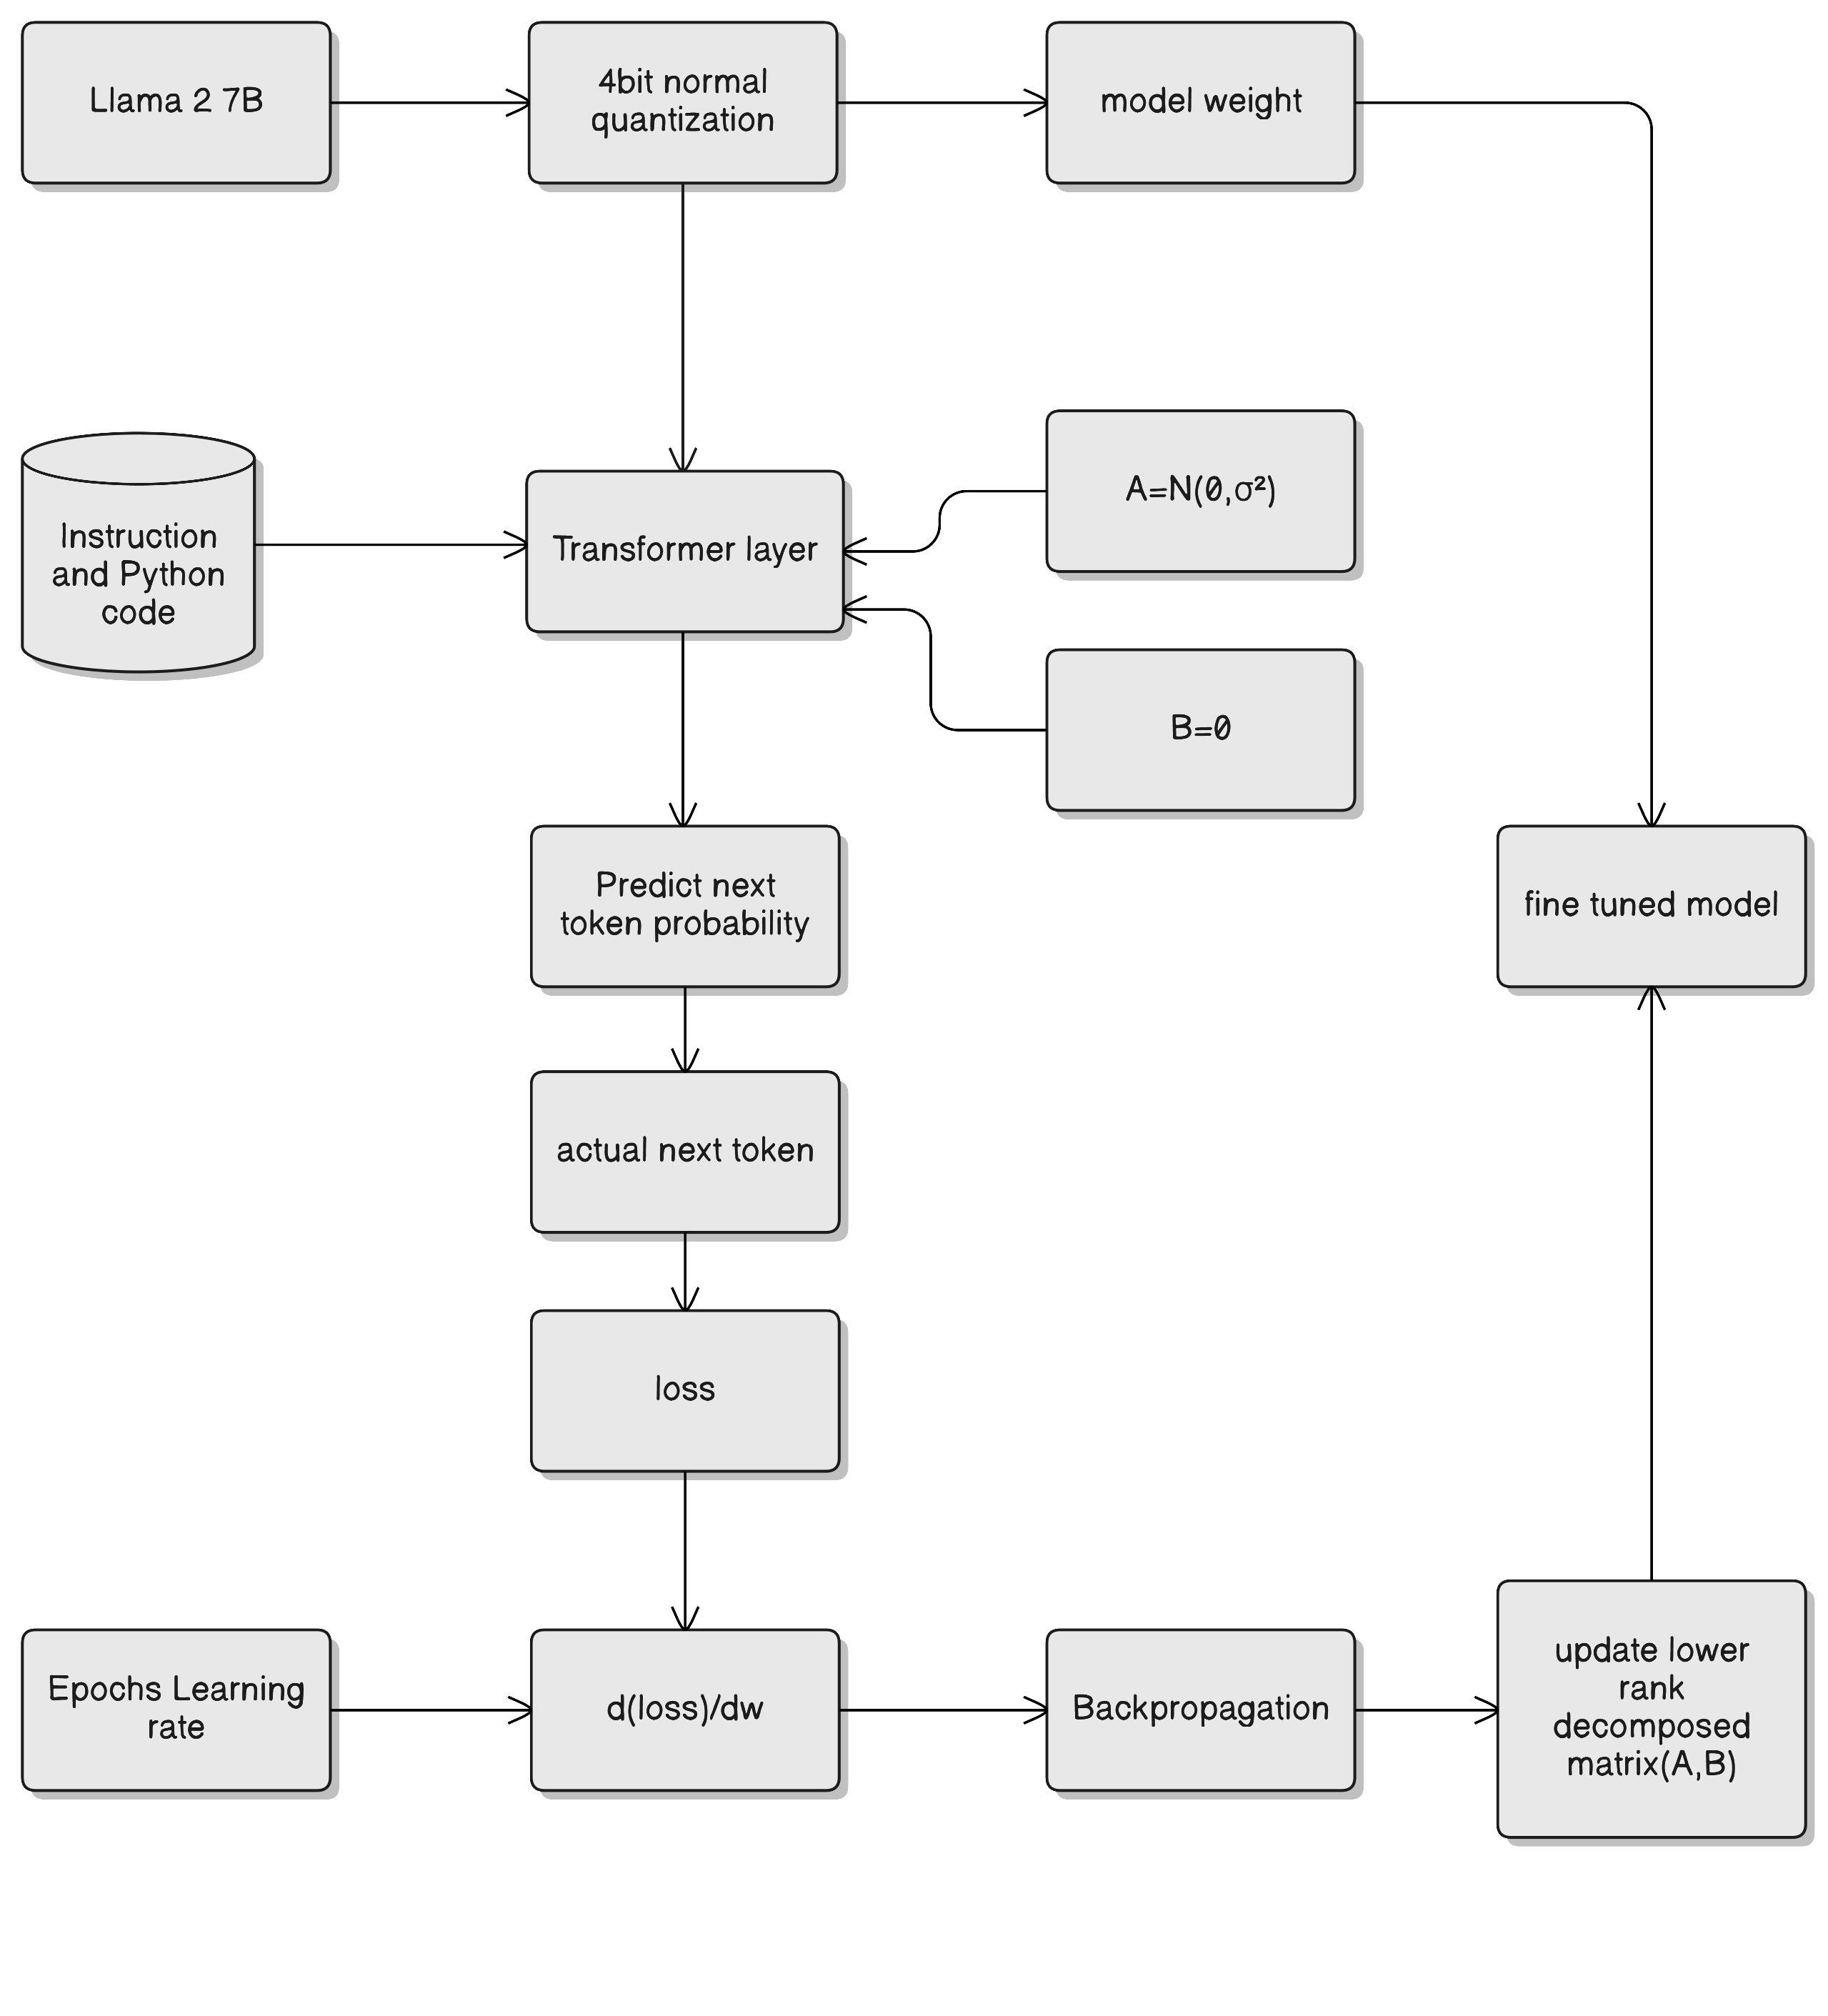
\includegraphics[width=1\linewidth]{flowdiagram.png} 
    \caption{Base Model Fine-tuning with QLoRA Adapter Layers}
    \label{fig:qlora_flow}
\end{figure}

\section{Evaluation Metrics}
Evaluation is split into functional correctness and similarity-based metrics.

\subsection{Functional Correctness}
Generated solutions are executed in a secure Docker sandbox and classified as:
\begin{itemize}
    \item \textbf{Right:} Passes all test cases.
    \item \textbf{Partial:} Passes some test cases.
    \item \textbf{Wrong:} Fails output or crashes.
\end{itemize}

\subsection{Automatic Similarity Metrics}
We utilize BLEU and CodeBLEU for quantitative assessment. CodeBLEU integrates structural information via Abstract Syntax Trees (AST) and data-flow:
\begin{equation}
\text{CodeBLEU} = \alpha \cdot \text{BLEU} + \beta \cdot \text{AST} + \gamma \cdot \text{DFScore} + \delta \cdot \text{SemanticScore}
\end{equation}
where $\alpha, \beta, \gamma, \delta$ are weighted parameters.
\chapter{IMPLEMENTATION DETAILS}

\section{Overview}
This project aims to fine-tune the Llama-2 7B large language model for Python code generation. 
The methodology is structured in three phases: dataset preparation, fine-tuning, and evaluation. 

\section{Data Collection and Preparation}
Fine-tuning Llama-2 7B for Python code generation requires a high-quality, domain-specific dataset 
containing diverse programming tasks and their corresponding solutions. 
We constructed a composite dataset from multiple reputable open-source sources.

\subsection{Dataset Sources}
\begin{table}[h!]
\centering
\caption{Datasets used for fine-tuning Llama-2 7B for Python code generation.}
\begin{tabular}{|p{3.5cm}|p{2cm}|p{5cm}|p{2.5cm}|}
\hline
\textbf{Dataset} & \textbf{Size} & \textbf{Description} & \textbf{License} \\
\hline
FlyTech Python Code Dataset (2025) & $\sim$42,000 pairs & Python scripts with comments, docstrings, and structured tasks. & MIT License \\
\hline
Python Code Instructions 18k & $\sim$18,000 pairs & Instruction prompts and Python responses (Alpaca-style). & CC BY-NC 4.0 \\
\hline
LeetCode (theabbie) & $\sim$2,318 files & Algorithmic reasoning and competitive programming files. & Public / Kaggle \\
\hline
LeetCode (gzipchrist) & $\sim$1,825 tasks & Detailed problem descriptions and difficulty levels. & Public / Kaggle \\
\hline
TACO Dataset & $\sim$26,000 tasks & Natural language tasks with executable Python solutions. & Apache 2.0 \\
\hline
\end{tabular}
\end{table}

\subsection{Preparation}
\textbf{Alpaca:} We used \texttt{qwen2.5-coder:1.5b} to identify whether the given rows were competitive programming (C.P.) problems. Approximately 12,000 problems were identified by the model, and we manually removed rows that were misclassified. The final dataset contained 11,926 rows of Python code with descriptions.  

\textbf{FlyTech:} We used [Details pending as per user request].

\textbf{TACO:} We used [Details pending as per user request].

\textbf{LeetCode Problems:} We compared the titles from the theabbie and gzipchrist datasets. A total of 1,204 matching problems were found. The first 175 problems were reserved for future Chain-of-Thought (CoT) tasks, leaving 1,029 rows for fine-tuning.

\subsection{Dataset Merging and Filtering}
All collected datasets were merged, resulting in a combined corpus of approximately 43,066 samples. The merged data were first filtered based on code length and repetition ratio to ensure quality and diversity:
\begin{itemize}
    \item Samples with code length greater than 7 tokens were retained.
    \item Samples with repetition ratio lower than 0.6 were retained.
\end{itemize}

After filtering, 39,823 samples remained. 

\subsection{Semantic Clustering and Sampling}
To further enhance dataset diversity, semantic clustering-based sampling was applied:
\begin{enumerate}
    \item Sentence embeddings were generated from the instruction text using the \texttt{all-MiniLM-L6-v2} transformer model.
    \item Embeddings were clustered into 20,000 clusters using MiniBatch K-Means.
    \item Clusters containing at least one row (effective clusters) numbered 18,526.
    \item For each cluster, the sample closest to the centroid was selected, producing a curated and semantically diverse final dataset.
\end{enumerate}

Among these, 1,860 rows were reserved for testing, and the remaining samples were used for fine-tuning and validation.
\chapter{PROJECT SCHEDULE}

% Tip: adjust the timeline and tasks below to match your plan.
% Use exact dates for tasks; calendar shows only months
\begin{table}[H]
	\centering
	\caption{Project schedule (Gantt chart)}
	\includegraphics[width=1\textwidth]{Planning.png}
	\label{fig:project_schedule}
\end{table}
\chapter{REMAINING TASKS}

\section{Final Model Training on Colab Pro}
The most critical remaining task is the fine-tuning of the Llama 2 7B model. 
\begin{itemize}
    \item \textbf{A100 GPU Utilization:} Due to the memory requirements of training on the full merged dataset, an NVIDIA A100 (40GB) in Colab Pro will be used.
    \item \textbf{Complete Dataset Run:} Training will proceed using the full integrated dataset (TACO, Alpaca-18k, Flytech) to ensure the model captures the nuances of all domains.
    \item \textbf{Checkpointing:} Implementing a robust checkpointing strategy to save model states at regular intervals to prevent data loss.
\end{itemize}

\section{Sandbox Evaluation and Inference}
A containerized sandbox will be used to host the model for final testing.
\begin{itemize}
    \item \textbf{Inference Testing:} Running the fine-tuned model against a diverse set of prompts in a Docker environment to measure response.
    \item \textbf{Qualitative Analysis:} The evaluation will focus on the model's ability to follow specific formatting requirements from the dataset that the base model may struggle with.
\end{itemize}

\section{Algorithmic Evaluation using CodeBLEU}
To provide a scientific basis for the model's coding capabilities, the project will implement CodeBLEU metrics.
\begin{itemize}
    \item \textbf{Syntactic and Semantic Analysis:} Evaluating generated code not just on word overlap but on Abstract Syntax Tree (AST) and data-flow similarity.
    \item \textbf{Benchmarking:} Comparing the CodeBLEU scores of our model against the base model to quantify the gains achieved through the TACO dataset.
\end{itemize}



% 5. BACK MATTER
\nocite{*}
\bibliographystyle{ieeetr}
\cleardoublepage
\phantomsection
\addcontentsline{toc}{chapter}{REFERENCES}
\bibliography{references} 

\end{document}